\subsection{Prototype}

From the list of features mentioned in the previous chapter we have selected the most important ones and created a prototype in a form of MVP (Minimum Viable Product). 

The selected features:

\begin{enumerate}
	\requirement{3}{load an Instruction}
	\requirement{3}{view the 3D representation of the Instruction step}
	\requirement{3}{switch to the next step in the Instruction}
	\requirement{3}{switch to the previous step in the Instruction}
	\requirement{3}{see the Transition between two Instruction steps}
	\requirement{2}{pause the Transition at any time}
	\requirement{2}{rewind the Transition}
	\requirement{2}{forward the Transition}
	\requirement{3}{rotate the Model in 3D space}
	\requirement{3}{zoom the Model in and out in 3D space}
	\requirement{1}{see creases of the Model} 
	\requirement{2}{distinguish paper's top and bottom sides} 
\end{enumerate}

Some of the listed functionalities require a numerical solver which is also included in the MVP.

Both Instructions and Transitions are represented using .fold files which we have extended with information required by the application.

\subsubsection{Frontend}

At first we had decided to use plain \tech{JavaScript} with the \tech{Rollup} bundler and \tech{Three.js} framework.
It quickly became apparent that the lack of state management will become problematic as the development progresses. Following that realization we have decided to incorporate a reactive framework - \tech{React} to aid the project with basic layout and aforementioned state manipulation. 
Due to minor interoperability issues the Rollup was also replaced with \tech{Webpack}.

The quality assurance is achieved through the use of:

\begin{description}
\item[Code linter] - EsLint
\item[Code prettiefier] - Prettier
\item[Test Runner] - Jest
\item[Continuous integration] - Github Actions
\end{description}

The implementation is continuously delivered to \tech{Netlify} via Github Actions.


\begin{figure}[H]
\caption{Origami simulation view}
  \centering
    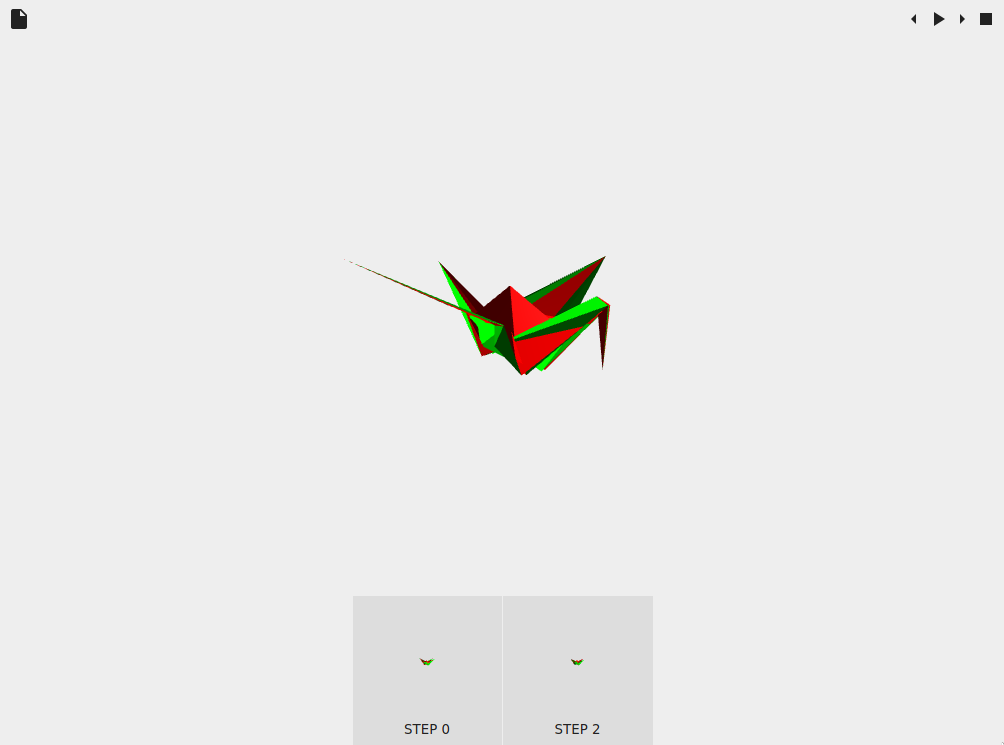
\includegraphics[width=0.8\textwidth]{assets/prototype-front.png}
\end{figure}

\subsubsection{Backend}

The current backend part is responsible for carrying out numerical computations.
It converts a provided Instruction into a set of coordinates representing
transitions between folding steps.\\

The solver is based on the techniques presented in the publication by A. Ghassaei.\cite{origami-simulator}.

The computational framework consists of the three most important forces,
that drive the folding process.

\begin{description}
	\item[Beam force] - responsible for preserving edge length
	\item[Face force] - responsible for preserving the original face shape
	\item[Crease force] - responsible for folding
\end{description}

Given the current vertices' positions, and the mountain-valley assignment,
the solver computes forces imposed on vertices, and calculates their next position
using the forward Euler integration.

An additional \textbf{damping force} is introduced to prevent solver from
high frequency oscilations, assuring numerical stability under most conditions.\\

The solver is implemented in \tech{python}, using \tech{numpy} and \tech{scipy} libraries. 


\begin{figure}[H]
	\caption{Visualization of vertices (dots), and forces applied to them (arrows)
	during folding of a rectangular sheet of paper in half, along the diagonal. }
  \centering
    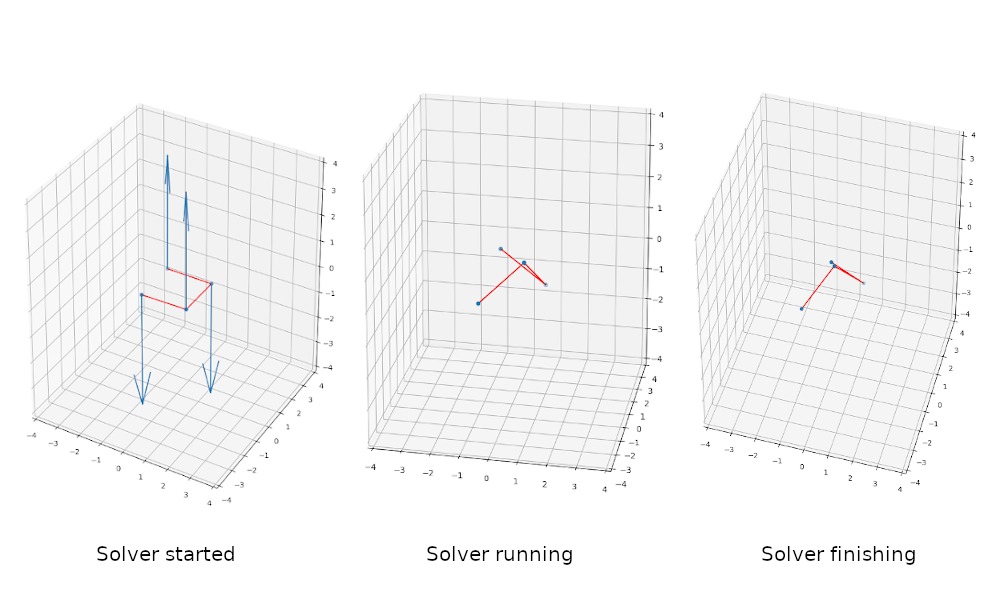
\includegraphics[width=0.8\textwidth]{assets/prototype-backend.png}
\end{figure}


\subsection{Project overview}
% Ogólny rzut na projekt - jakie są jego główne moduły, komponenty? Koniecznie rysunek z komentarzem. Koniecznie zasada działania, jeśli potrzebna. Mile widziane rysunki koncepcyjne. %

\subsection{Technology stack}
% Stos technologiczny - jaki jest, z opisem do czego poszczególne elementy, z komentarzem czemu taki i co było brane pod uwagę, tutaj może być opis ew. prototypów technologicznych jako wyjaśnienie. Ew. w dokumentacji procesowej z odwołaniem w tym miejscu. Jeśli wykorzystaliście jakieś specyficzne narzędzie np. do tworzenia gier to warto poświecić nieco więcej miejsca i opisać co z niego wykorzystaliście i jak ono działa i co daje. %

\subsection{Components overview}
% Przegląd poszczególnych komponentów a wiec np. baza danych, aplikacja typu klient, serwis RESTowy. Jeśli baza to ERD z opisem, jeśli aplikacja kliencka to jakie elementy, widoki, jak się łączy i kiedy. Jeśli prosta aplikacja WWW to można pokazać strukturę projektu. Jeśli serwis RESTowy to jego specyfikacja z przykładami. Protokół komunikacji to może być zupełnie osobny opis. %

\subsection{Algorithms}
% Ciekawsze algorytmy, aspekty, mechanizmy np. logowanie, indeksowane, cachowanie, synchronizacja, backup, jakieś procesy w tle, jakieś progress bary, jakieś analizy, generowanie warstw GISowych, lokalizacja etc. Jest tu często o czym pisać. %

\subsection{Development environment setup}
% Instrukcja postawienia środowiska deweloperskiego - jeśli potrzeba wypełniacza %

\subsection{Quality assurance}
% Quality Assurance: czy mamy testy jednostkowe? Czy mamy inne testy automatyczne? Jakich bibliotek używacie? %

\subsection{Problems encountered}
% Z jakimi problemami technicznymi sie borykaliście? Jeśli nie opisaliście ich w dokumentacji procesowej. %

